Z punktu widzenia matematyków różnica pomiędzy 1.0000000000000001 a 1.0 jest spora, ponieważ pomiędzy tymi wartościami mamy nieskończenie wiele liczb, natomiast przy obliczeniach, których dokonujemy używając maszyn cyfrowych musimy zważyć, czy zwiększać dokładność zwiększając ilość bitów zajmowanych przez liczby, jednocześnie zmniejszać szybkość operacji, czy wykorzystać mniej dokładne reprezentacje zyskując na szybkości pewnych operacji. 

\section{Kodowanie}
Najczęściej używaną reprezentacją liczb rzeczywistych jest opisana przez normę IEEE 754. Norma ta definiuje zapis liczby w 32, 64 liczb 128 bitach. W językach programowania dostępne jako klasy \textit{Float}, \textit{Double}. 



\begin{itemize}
    \item Matlab: przypisanie a=1.0000000000000001 //  a=1;
    \item Python: print (.000600000000000000001) // 0.0006. 
    \item Java: \(0.1 + 0.2 = 0.30000000000000004.\)
\end{itemize}

Do zastosowań specjalnych możemy użyć specjalnych formatów zapisu np. BigDecimal w Java o~większej dokładności (większej liczbie cyfr znaczących), lecz o~dużo dłuższym czasie operacji.  
\newline
Float - 0.002 [sek.] / BigDecimal 0.042 [sek.]

\break

\section{operacje równoległe}
operacje niezależne - na rysunku oznaczone kolorem zielonym - takie jak mnożenie wag przez wartości wejściowe możemy wykonywać równolegle, wykorzystując osobne wątki, procesy, rdzenie. Operacje sumowania nie są operacjami niezależnymi. 

\begin{figure}[h]
	\centering 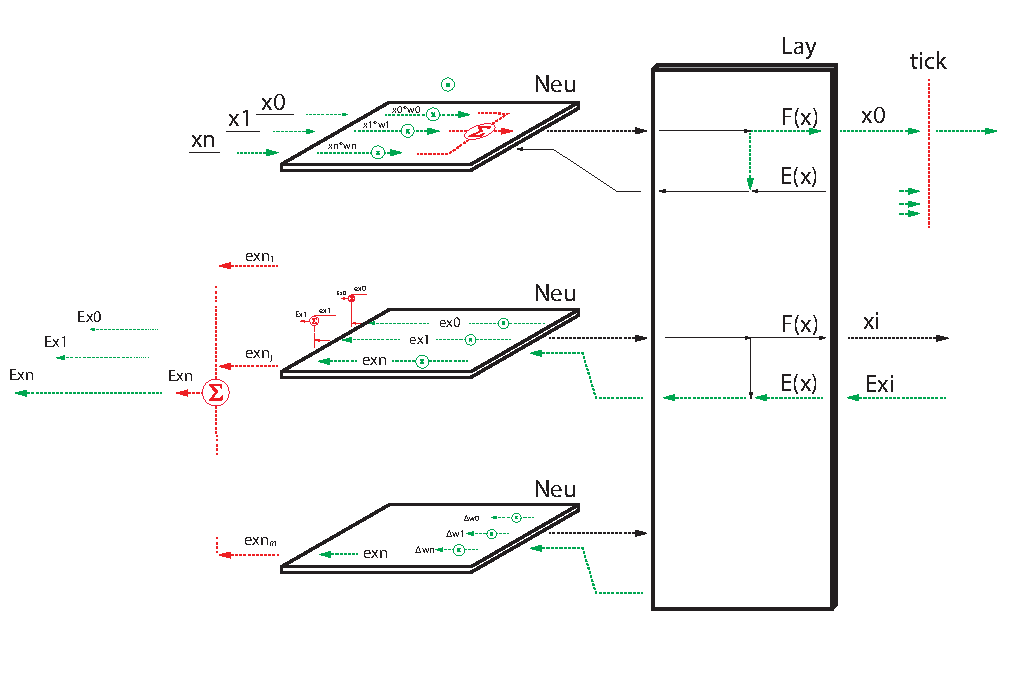
\includegraphics[width=0.9\textwidth]{gfx/3drev.pdf} 
	\caption{ operacje niezależne i operacje wymagające synchronizacji}
	\label{rys:operacjesynch}
\end{figure}


Sumowanie a+b+c+d realizowana jest analogiczne do zdegenerowanego drzewa binarnego czyli 
(((a+b)+c)+d)... nie jest operacją równoległą. Przy dużej ilości składników możemy spróbować zastosować zwykłe drzewo binarne nie zdegenerowane, a operacja dodawania może stanie się częściowo równoległa  ( (a+b)  +  (c+d) ... ).
Maszyny cyfrowe obecnie nie są wyposażone w sumatory wielokanałowe pozwalające dodawać więcej niż 2 liczby jednocześnie. Najprostsza realizacja fizyczna takiego sumatora jest możliwa do realizacji w układach FPGA, można także zastosować nawiasy.

\begin{figure}[h]
	\centering 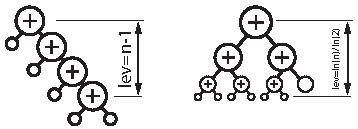
\includegraphics[width=0.7\textwidth]{gfx/sum.pdf} 
	\caption{ drzewo zdegenerowane i niezdegenerowane}
	\label{rys:operacjesynch}
\end{figure}

\break

 
\section{Dodawanie równoległe}
różnice w szybkości dodawania: (C++) 
\begin{equation*}
b=a1+a2+a3+a4+...+a1024;
\end{equation*}
czas wykonania: \textbf{0.247875 [sek.]}

\begin{equation*}
b=((..((a1+a2)+(a3+a4))+((a5+a6) ...
\end{equation*}
czas wykonania: \textbf{0.09568 [sek.]} 
\newline 
\newline Ponad dwukrotne zwiększenie szybkości przez dodanie nawiasów. 
przy 32 składnikach mamy 16 + 8 + 4 + 2 + 1 dodawań, jednak pierwsze 16 może być wykonane równolegle, kolejna 8 także jest od siebie niezależna, podobnie 4 i 2. Czyli dla 32 elementów  mamy 31 dodawań w 5 poziomach. Dla 1024 składników mamy 1023 dodawania, 512+256+128...+1 w 10 poziomach. Podsumowując 1023 dodawania możemy wykonać w czasie takim jak 10 dodawań korzystając z osobnych 512 rdzeni CUDA zakładając że dostęp do pamięci będzie niezależny. Korzystając ze zwykłego CPU poszczególne rdzenie będą czekały się w kolejce po odczyt wartości składników oraz w drugiej kolejce do zapisu wyników w pamięci. Jeśli kod będzie "optymalizowany" np. przez procesor i zmieni się kolejność niektórych działań, wynik sumowania może być nieprawidłowy.

\section{ Wątki }
Rozdzielenie przetwarzania w ramach procesu na wątki umożliwia równoległe przetwarzanie danych i jest wspierane przez nowoczesne procesory. Proces będzie miał do dyspozycji kilka niezależnych jednostek liczących ALU, więc niezależne operacje będą wykonywane w tym samym czasie. A zatem pojedyncze mnożenie zajmie tyle czasu co kilka mnożeń na kilku rdzeniach. 

\section{ HyperWątki HT}
Technologia wprowadzone przez Inter HyperThread(R) tworzy dwie kolejki rozkazów dla jednego rdzenia, co dla systemu operacyjnego wygląda na dwa niezależne rdzenie. W rezultacie w czasie gdy jedna kolejka wykorzystuje jednostkę liczącą, w drugiej kolejce może być bez przeszkód wykonana instrukcja odczytania lub zapisu danych do pamięci - a te instrukcje zajmują nawet kilkanaście cykli zegara. W tej sytuacji mamy zwiększone wykorzystanie potencjału pojedynczego rdzenia. 

\section{ Pamięć operacyjna }
Ponieważ dostęp do \textit{magistrali pamięci} jest synchroniczny, to nawet jeśli samo przetwarzanie przez ALU będzie równoległe, to odczyt i zapis w pamięci będzie miał charakter zbliżony do synchronicznego. Nawet przy dwu niezależnych kanałach po 128 bitów w każdym (DDR5). 

\section{ Rdzenie CUDA }
Procesory ogólnego przeznaczenia, mimo wielu wysiłków, nie są w stanie zapewnić w pełni równoległego przetwarzania. Równoległe przetwarzanie mogą zapewnić np. procesory graficzne, w których znajduje się wiele jednostek obliczeniowych, ale przede wszystkim dostęp do pamięci jest rzeczywiście równoległy. Procesory graficzne projektowane były do obliczeń translacji punktów w przestrzeni, a operacje te sprowadzały się do mnożenia macierzy współrzędnych znormalizowanych punktu przez macierz translacji:

\begin{equation*}
  T =  \begin{bmatrix}
 1 & 0 & 0 & x\\
 0 & 1 & 0 & y\\
 0 & 0 & 1 & z\\
 0 & 0 & 0 & 1
        \end{bmatrix} ,
  O_x =  \begin{bmatrix}
 1 & 0 & 0 & 0\\
 0 & c & -s & 0\\
 0 & s & c & 0\\
 0 & 0 & 0 & 1
        \end{bmatrix} ,
R =  \begin{bmatrix}
 1 & 0 & 0 & 0\\
 0 & 1 & 0 & 0\\
 0 & 0 & 1 & 0\\
 0 & 0 & 1/d & 0
        \end{bmatrix} 
\end{equation*}

a po rozpisaniu mamy:
\begin{equation*}
\begin{matrix}
  X - x*m[0][0] + y*m[1][0]+z*m[2][0] + w*m[3][0] \\

  Y - x*m[0][1] + y*m[1][1]+z*m[2][1] + w*m[3][1] \\

  Z - x*m[0][2] + y*m[1][2]+z*m[2][2] + w*m[3][2] \\

  W - x*m[0][3] + y*m[1][3]+z*m[2][3] + w*m[3][3]  \\
  \end{matrix}
\end{equation*}

i są to te same obliczenia, które wykonujemy wielokrotnie podczas pracy z matematycznymi modelami sieci neuronowych:
\begin{equation*}
  y - x_0*w_0 + x_1*w_1 +x_2*w_2 ... +x_2*w_2;
\end{equation*}
a jeśli będą one wykonane przez osobne rdzenie CUDA, a wyniki będą zapisane w pamięci VRam o dostępnie równoległym - wtedy wiele takich operacji zajmie dokładnie tyle samo czasu co pojedyncza operacja. Idealnie byłoby gdyby cała praca odbywała się w VRAM i na rdzeniach CUDA bez konieczności przesyłania danych w każdym cyklu do pamięci operacyjnej RAM. Jeśli zbiór danych w całości znajdowałby się w VRAM, to przejście sygnałów przez jedną warstwę sieci trwałoby tyle co jedna operacja, a propagacja przez sieć trwałaby tyle razy dłużej ile warstw mamy w sieci. Powrót sygnału w postaci wielkości błędu podobnie zajmowałby mniej więcej tyle czasu. (O ile operacje mnożenia możemy wykonać równolegle to operacje wielokrotnego dodawania już nie do końca). 
Równoległe zmiany kilku wag również byłyby dokonywane w takim czasie jak zmiana pojedynczej wagi.
\newline
Wprowadzanie na rynek gier sieciowych wymagających do zabawy coraz wydajniejszych kart graficznych oraz pojawienie się wirtualnych walut typu Bitcoin wydobywanych - obliczanych właśnie przy użyciu takiego sprzętu zwiększyła zapotrzebowanie na coraz wydajniejsze jednostki mimo sporych kosztów jak dla użytkownika indywidualnego. 
\newline
Dostępność cenowa coraz wydajniejszych jednostek, które przyspieszają obliczenia nawet o kilka rzędów wielkości, spowodowała, że budowanie prawdziwie używalnych modeli stało się możliwe. A temat \textit{„sztucznej inteligencji”} znany wcześniej jedynie garstce naukowców, stał się nagle tematem bardzo popularnym. 

\section{Matlab}
Dodatek Parallel computing w Matlab umożliwia wykonywanie obliczeń równolegle, w osobnych wątkach, procesach a także z wykorzystaniem kart graficznych (obecnie tylko NVidia). Dodatki Optimalization Toolbox i Optimalization Computing Toolbox optymalizują tworzony kod zwiększając jego wydajność. Dodatek Deep Learning Toolbox dostarcza gotowych metod do obliczeń sieci neuronowych.

\section{Python}
Metody do obliczeń sieci neuronowych w języka Python dostarczone są w bibliotekach scikit-learn i TensorFlow2 a dostarczają one gotowych metod przydatnych w obliczeniach sieci neuronowych. Wykorzystują one możliwości równoległego przetwarzania, które oferuje sprzęt na którym uruchamiany jest kod.

https://www.geeksforgeeks.org/matplotlib-tutorial/
matlabplotlib 